% !TeX TS-program = lualatex
\documentclass[12pt,letterpaper]{article}
%%% LuaLaTex
\usepackage{fontspec}
\usepackage{amsmath}% if desired
\usepackage{unicode-math}
\renewcommand{\boldsymbol}{\symbf}

\setmainfont{TeX Gyre Pagella}[
Numbers	=	{OldStyle, Proportional},
Ligatures	=	TeX,
%Script=Arabic
%Contextuals = WordFinal,	
]
\setsansfont{TeX Gyre Adventor}[
Numbers	=	{OldStyle, Proportional},
Ligatures	=	TeX,
Scale=MatchLowercase]
\setmonofont{Inconsolata}[
Scale = MatchLowercase, 
Ligatures = TeX,
]
\setmathfont{XITS Math}
\setmathfont[range=it->up]{Neo Euler}
\setmathfont[range=up/{num}]{Neo Euler}
\newfontface{\andm}{Andale Mono}
\newfontface{\babm}{BabelStone Mayan Numerals}%{Symbola}
\newfontface{\mayanumerals}{BabelStone Mayan Numerals}
\newfontface{\charis}{Charis SIL}%{Gentium Plus}
\newfontface{\charisbf}{Charis SIL Bold}%{Charis SIL}
%\newfontface{\palarab}{PalatinoLTArabic}%{Gentium Plus}
%%%%%%%%%%%%
\linespread{1.05}% Palatino needs more leading (space between lines) {1.01} {1.08}
%\usepackage{ucs}
\usepackage[spanish,mexico]{babel}
%\usepackage{amsmath}
%\usepackage{amsfonts}
%\usepackage{amssymb}
%\usepackage{makeidx}
\usepackage[format=hang,font=small,labelfont=bf,labelsep=quad]{caption}
\usepackage{xcolor}
\usepackage{graphicx}
\usepackage[useregional]{datetime2}
\usepackage{fancyhdr}
\usepackage{tikz}
\usepackage[colorlinks=true,urlcolor=brown]{hyperref}
% % % %Geometry
\usepackage{geometry}%\usepackage[showframe]{geometry}
%\usepackage{layout}
\setlength{\voffset}{-0.7in}
\setlength{\headsep}{10pt}
\setlength{\textheight}{10.5in}
%\usepackage{coloremoji}
\usepackage{wasysym} %emoticons :)
\newcommand{\LuaLaTeX}{L\kern-0.25em\raise0.5ex\hbox{\tiny U}\kern-0.04em\raise0.5ex\hbox{\tiny A}\kern-0.05em\LaTeX}
\newcommand{\fej}{\relax\hfill\ifmmode{\lower.5ex\hbox{{\textcolor{blue}{\LARGE\smiley al 15pt}}}}\else\lower.5ex\hbox{{\textcolor{blue}{\LARGE \smiley}}}}  % Smiley emoticon :)
\author{\textsc{Manuel López Mateos}}
%%  Noviembre 16, 2019
% % % % % % % Para usar título, autor y fecha por separado.
\makeatletter
\let\newtitle\@title
\let\elautor\@author
\let\newdate\@date
\makeatother
%
%
% % % % Enviroments
\newenvironment{definition}[1][Definición.]{\begin{trivlist}
\item[\hskip \labelsep {\bfseries #1}]}{\end{trivlist}}
% % % % % % % % % % % %
%
% % % % % % % % Headers
\pagestyle{fancy}
\fancyhf{}
\rhead{\color{olive}\hfill \DTMnow}
\lhead{\color{olive}\elautor}
\cfoot{\thepage}
\renewcommand{\headrule}{\color{olive}\hrule}
\newcommand{\R}{\relax\ifmmode\mathbb{R}\else${\mathbb{R}}$\fi}
%\rfoot{}
% % % % % % %
\begin{document} %\layout
\bigskip 

\noindent Los puntos $A=(-2,4)$, $B=(-3,-2)$ y $C=(6,-1)$ en el plano $\R^2$ definen el $\triangle ABC$. Encuentra la ecuación de la recta que contiene a la \emph{\color{purple}altura} $\overline{AJ}$ que pasa por el vértice $A$, según se muestra en la figura.
\begin{figure}[ht]
	\centering
	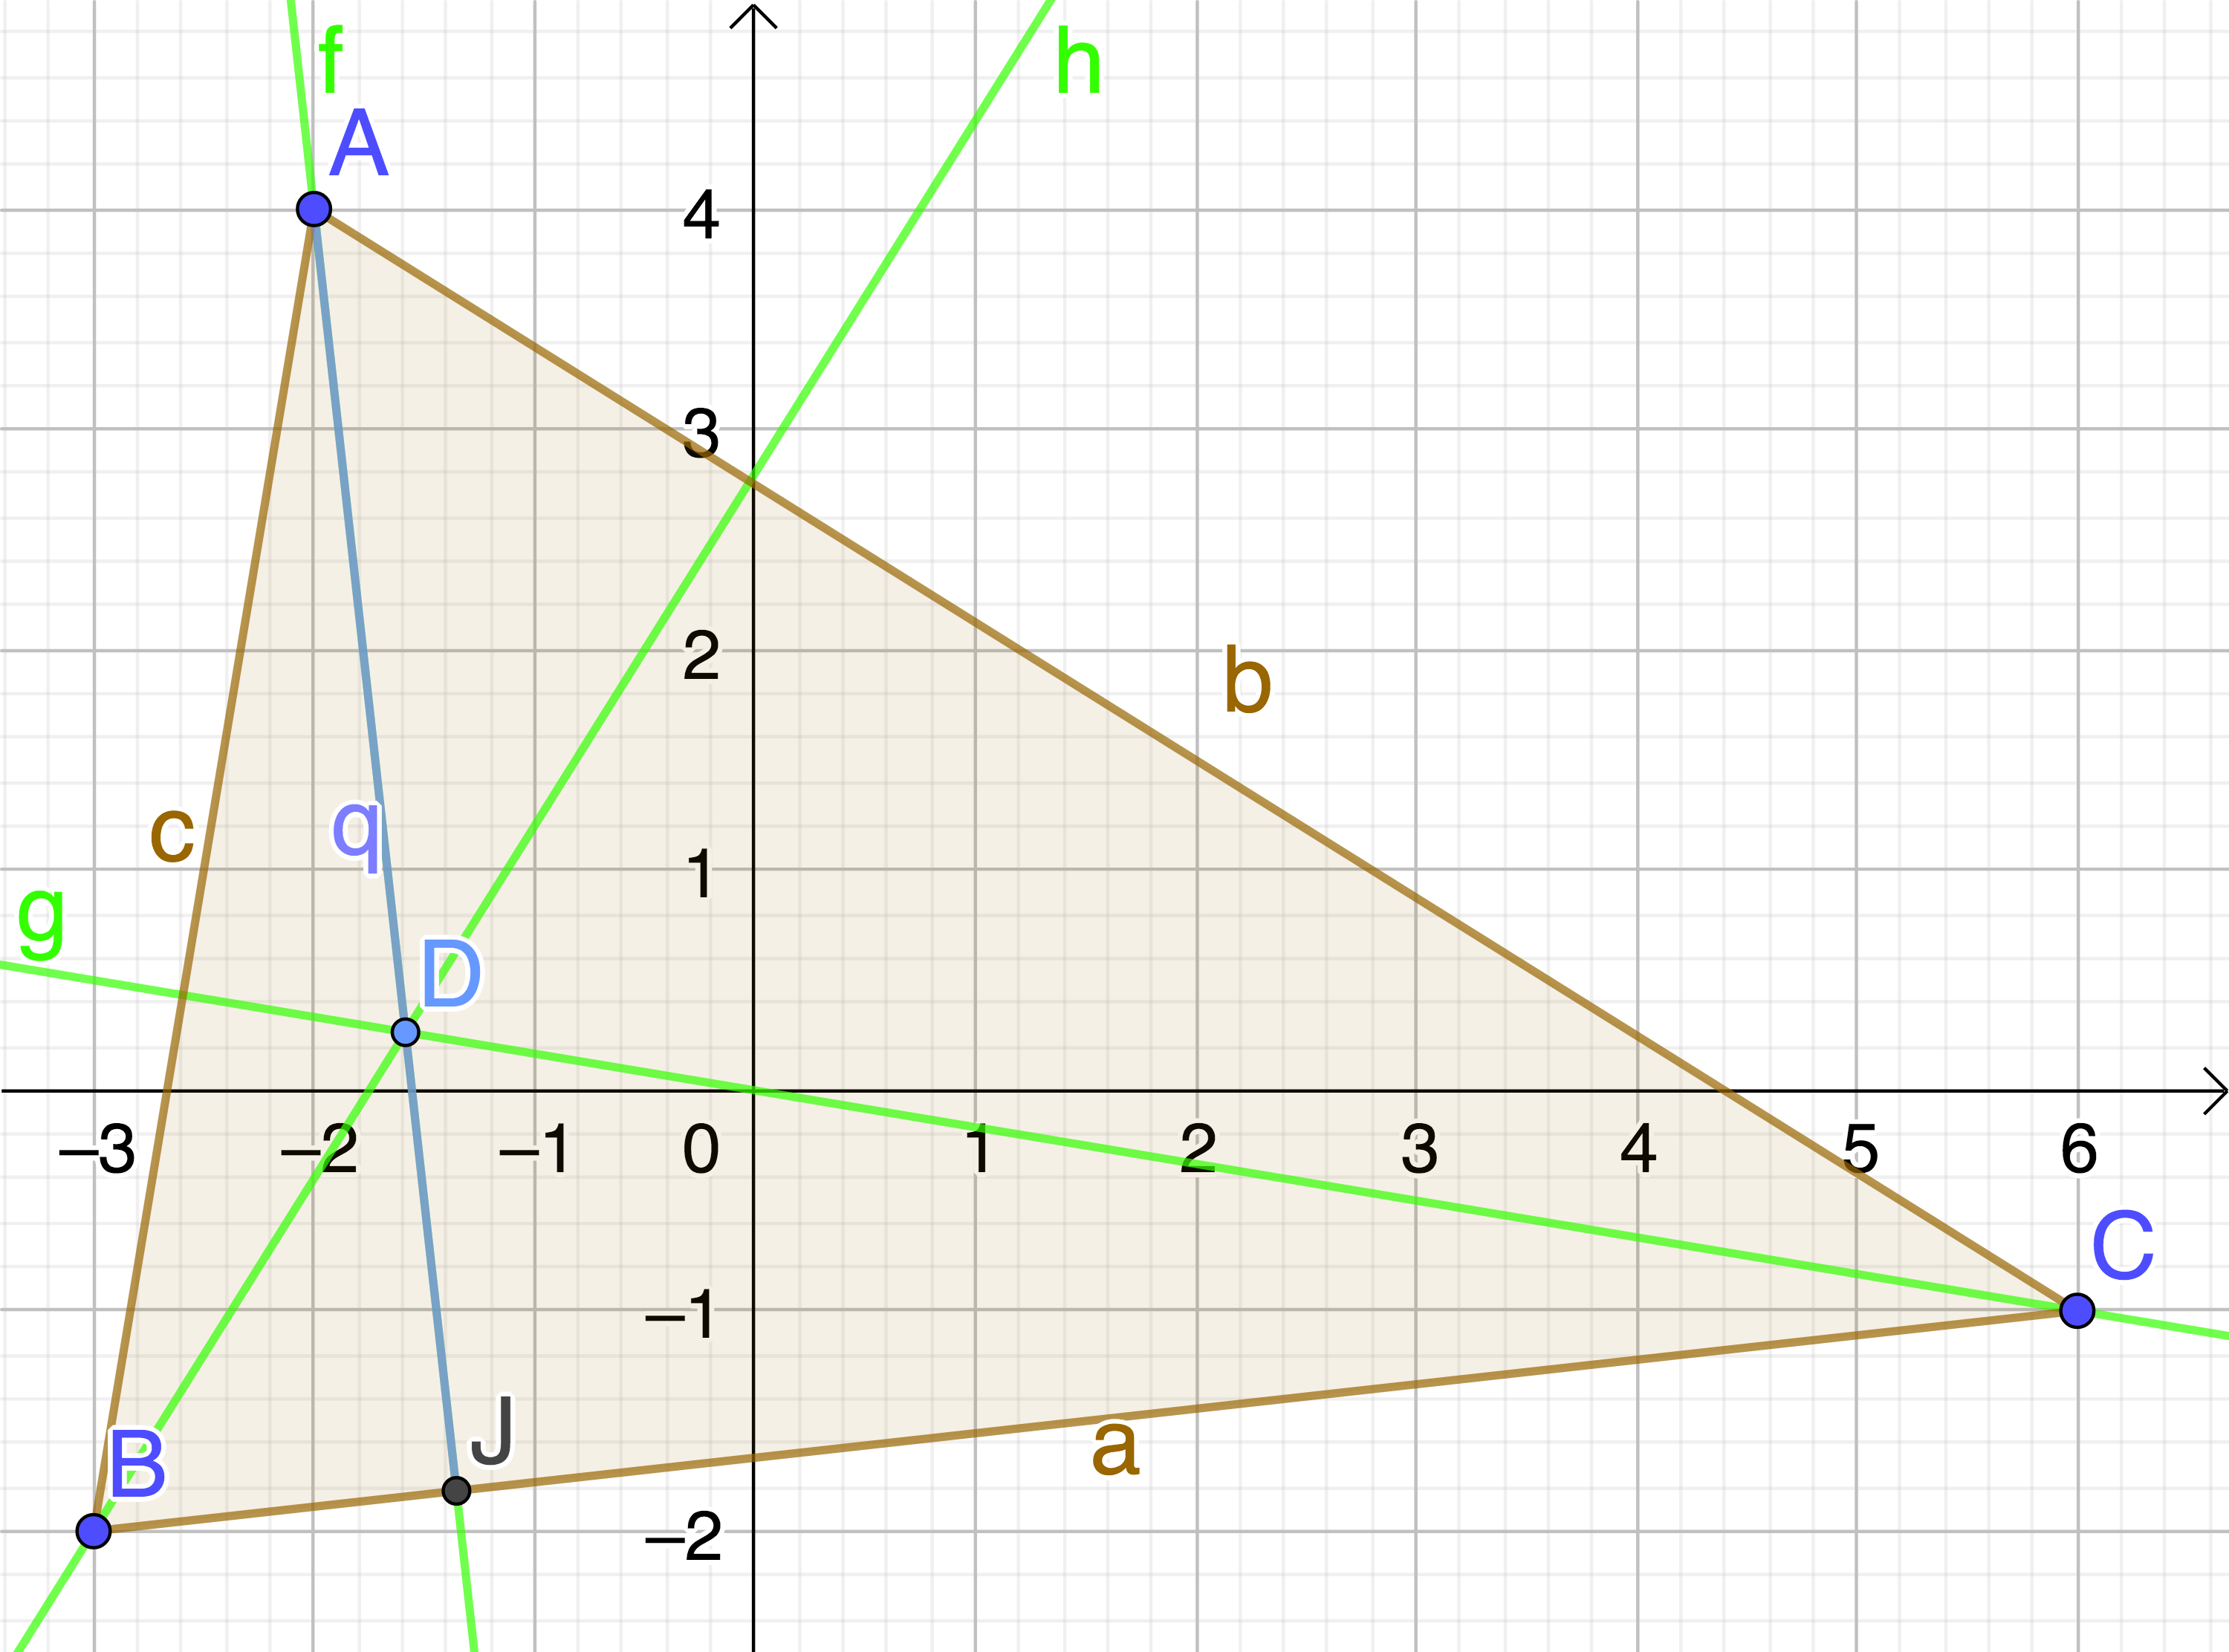
\includegraphics[scale=0.8]{img/altura-triangb.png}
	\caption{La \emph{altura} (en azul) que pasa por $A$, es perpendicular  al lado $a$.}\label{fig:altura}
\end{figure}

Las \textbf{\color{purple}alturas} de un triángulo son \emph{\color{purple}segmentos} que van de un vértice a la base de la perpendicular al lado opuesto. Así, la \emph{altura} correspondiente al vértice $A$ es el segmento $\overline{AJ}$, donde $J$ es la base de la perpendicular al lado $a$, que pasa por $A$. 

Las \emph{tres} \emph{alturas} se \emph{\color{purple}intersecan} en un punto, llamado \textbf{\color{purple}ortocentro} del triángulo.

Como la recta que contiene al lado $a$ pasa por los puntos $B$ y $C$, entonces tiene pendiente
$$m_1=\frac{-1-(-2)}{6-(-3)}=\frac{1}{9}.$$

Si una recta $L$ tiene pendiente $m_1$, cualquier recta perpendicular a $L$ tiene pendiente $m_2$ tal que $m_1m_2=-1$.

La pendiente $m_2$ de una recta perpendicular a $a$ (con pendiente $m_1$) cumple que $m_1m_2=-1$, luego $m_2=-9$.

Luego la ecuación de la perpendicular a $a$ es de la forma
$$y=-9x+b,$$
donde $b$ es tal que la recta pase por el vértice $A$, para hallar $b$, substituimos en la ecuación anterior las coordenadas de $A=(-2,4)$,
$$4=-9(-2)+b,\quad\text{de donde}\quad b=4-18=-14.$$
Así, la ecuación buscada, de la recta que contiene a la \emph{altura}, en su forma canónica, es
\[y=-9x-14.\tag*{\fej}\]

Expresa la ecuación en su forma general. 

Para hallar el \textbf{\color{purple}ortocentro del triángulo}, encuentra la ecuación de la recta que contenga a \emph{otra} \emph{altura}, por ejemplo, la que pasa por $B$. Después calcula la intersección de esas dos rectas. El punto hallado es el \emph{ortocentro}.

Las coordenadas del punto hallado deben satisfacer la ecuación de la recta que contiene a la \emph{tercera altura}.
\vfill

\begin{center}
	\texttt{\color{brown}Solución en}\enspace \url{https://www.geogebra.org/classic/mettdtne}
\end{center}


\begin{center}
	{\footnotesize\color{olive} Esta hoja se formó con el sistema \LuaLaTeX. La gráfica con \textsc{Geogebra}.}
\end{center}
\end{document}